% Exact Selberg weights for the integers at y=10. Bar heights are lambda_d.
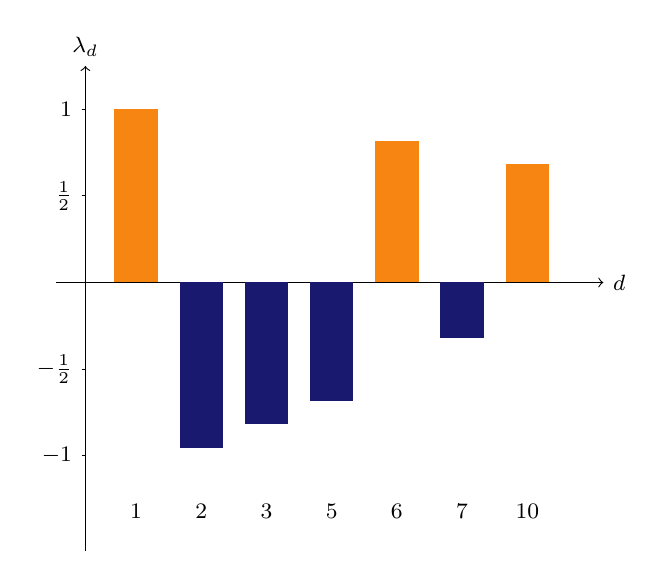
\begin{tikzpicture}[x=0.92cm,y=2.2cm,every node/.style={font=\footnotesize}]
  \draw[->] (-0.4,0)--(7.15,0) node[right] {$d$};
  \draw[->] (0,-1.55)--(0,1.25) node[above] {$\lambda_d$};
  \draw (0,1)--(-0.05,1) node[left] {$1$};
  \draw (0,0.5)--(-0.05,0.5) node[left] {$\frac12$};
  \draw (0,-0.5)--(-0.05,-0.5) node[left] {$-\frac12$};
  \draw (0,-1)--(-0.05,-1) node[left] {$-1$};
  \fill[BurntOrange] (0.40,0) rectangle (1.00,1);
  \fill[MidnightBlue] (1.30,0) rectangle (1.90,-0.9545);
  \fill[MidnightBlue] (2.20,0) rectangle (2.80,-0.8182);
  \fill[MidnightBlue] (3.10,0) rectangle (3.70,-0.6818);
  \fill[BurntOrange] (4.00,0) rectangle (4.60,0.8182);
  \fill[MidnightBlue] (4.90,0) rectangle (5.50,-0.3182);
  \fill[BurntOrange] (5.80,0) rectangle (6.40,0.6818);
  \node at (0.70,-1.32) {$1$};
  \node at (1.60,-1.32) {$2$};
  \node at (2.50,-1.32) {$3$};
  \node at (3.40,-1.32) {$5$};
  \node at (4.30,-1.32) {$6$};
  \node at (5.20,-1.32) {$7$};
  \node at (6.10,-1.32) {$10$};
\end{tikzpicture}
